%%%%%%%%%%%%%%%%%%%%%%%%%%%%%%%%%%%
%This is the LaTeX ARTICLE template for RSC journals
%Copyright The Royal Society of Chemistry 2016
%%%%%%%%%%%%%%%%%%%%%%%%%%%%%%%%%%%

\documentclass[twoside,twocolumn,9pt]{article}
\usepackage{extsizes}
\usepackage[super,sort&compress,comma]{natbib} 
\usepackage[version=3]{mhchem}
\usepackage[left=1.5cm, right=1.5cm, top=1.785cm, bottom=2.0cm]{geometry}
\usepackage{balance}
\usepackage{mathptmx}
\usepackage{sectsty}
\usepackage{graphicx} 
\usepackage{lastpage}
\usepackage[format=plain,justification=justified,singlelinecheck=false,font={stretch=1.125,small,sf},labelfont=bf,labelsep=space]{caption}
\usepackage{float}
\usepackage{fancyhdr}
\usepackage{fnpos}
\usepackage[english]{babel}
\addto{\captionsenglish}{%
  \renewcommand{\refname}{Notes and references}
}
\usepackage{array}
\usepackage{droidsans}
\usepackage{charter}
\usepackage[T1]{fontenc}
\usepackage[usenames,dvipsnames]{xcolor}
\usepackage{setspace}
\usepackage[compact]{titlesec}
\usepackage{hyperref}
%%%Please don't disable any packages in the preamble, as this may cause the template to display incorrectly.%%%


\usepackage{epstopdf}%This line makes .eps figures into .pdf - please comment out if not required.

\definecolor{cream}{RGB}{222,217,201}

\usepackage{layout}

\begin{document}

\pagestyle{fancy}
\thispagestyle{plain}
\fancypagestyle{plain}{
%%%HEADER%%%
\renewcommand{\headrulewidth}{0pt}
}
%%%END OF HEADER


%%%PAGE SETUP - Please do not change any commands within this section%%%
\makeFNbottom
\makeatletter
\renewcommand\LARGE{\@setfontsize\LARGE{15pt}{17}}
\renewcommand\Large{\@setfontsize\Large{12pt}{14}}
\renewcommand\large{\@setfontsize\large{10pt}{12}}
\renewcommand\footnotesize{\@setfontsize\footnotesize{7pt}{10}}
\makeatother

\renewcommand{\thefootnote}{\fnsymbol{footnote}}
\renewcommand\footnoterule{\vspace*{1pt}% 
\color{cream}\hrule width 3.5in height 0.4pt \color{black}\vspace*{5pt}} 
\setcounter{secnumdepth}{5}

\makeatletter 
\renewcommand\@biblabel[1]{#1}            
\renewcommand\@makefntext[1]% 
{\noindent\makebox[0pt][r]{\@thefnmark\,}#1}
\makeatother 
\renewcommand{\figurename}{\small{Fig.}~}
\sectionfont{\sffamily\Large}
\subsectionfont{\normalsize}
\subsubsectionfont{\bf}
\setstretch{1.125} %In particular, please do not alter this line.
\setlength{\skip\footins}{0.8cm}
\setlength{\footnotesep}{0.25cm}
\setlength{\jot}{10pt}
\titlespacing*{\section}{0pt}{4pt}{4pt}
\titlespacing*{\subsection}{0pt}{15pt}{1pt}
%%%END OF PAGE SETUP%%%

%%%FOOTER%%%
\fancyfoot{}
\fancyfoot[LO,RE]{\vspace{-7.1pt}
\includegraphics[height=9pt]{auxiliary/rsc_template_head_foot/LF}}
\fancyfoot[CO]{\vspace{-7.1pt}\hspace{13.2cm}
\includegraphics{auxiliary/rsc_template_head_foot/RF}}
\fancyfoot[CE]{\vspace{-7.2pt}\hspace{-14.2cm}
\includegraphics{auxiliary/rsc_template_head_foot/RF}}
\fancyfoot[RO]{\footnotesize{\sffamily{1--\pageref{LastPage} ~\textbar  \hspace{2pt}\thepage}}}
\fancyfoot[LE]{\footnotesize{\sffamily{\thepage~\textbar\hspace{3.45cm} 1--\pageref{LastPage}}}}
\fancyhead{}
\renewcommand{\headrulewidth}{0pt} 
\renewcommand{\footrulewidth}{0pt}
\setlength{\arrayrulewidth}{1pt}
\setlength{\columnsep}{6.5mm}
\setlength\bibsep{1pt}
%%%END OF FOOTER%%%

%%%FIGURE SETUP - please do not change any commands within this section%%%
\makeatletter 
\newlength{\figrulesep} 
\setlength{\figrulesep}{0.5\textfloatsep} 

\newcommand{\topfigrule}{\vspace*{-1pt}% 
\noindent{\color{cream}\rule[-\figrulesep]{\columnwidth}{1.5pt}} }

\newcommand{\botfigrule}{\vspace*{-2pt}% 
\noindent{\color{cream}\rule[\figrulesep]{\columnwidth}{1.5pt}} }

\newcommand{\dblfigrule}{\vspace*{-1pt}% 
\noindent{\color{cream}\rule[-\figrulesep]{\textwidth}{1.5pt}} }

\makeatother
%%%END OF FIGURE SETUP%%%

%%%TITLE, AUTHORS AND ABSTRACT%%%
\twocolumn[
  \begin{@twocolumnfalse}
{
\includegraphics[height=30pt]{auxiliary/rsc_template_head_foot/journal_name}\hfill\raisebox{0pt}[0pt][0pt]{
\includegraphics[height=55pt]{auxiliary/rsc_template_head_foot/RSC_LOGO_CMYK}}\\[1ex]

\includegraphics[width=18.5cm]{auxiliary/rsc_template_head_foot/header_bar}}\par
\vspace{1em}
\sffamily
\begin{tabular}{m{4.5cm} p{13.5cm} }


\includegraphics{auxiliary/rsc_template_head_foot/DOI} & \noindent\LARGE{\textbf{Rapid technological progress in white light-emitting diodes and its sources in innovation and technology spillovers}} \\
\vspace{0.3cm} & \vspace{0.3cm} \\

 & \noindent\large{Michael Weinold \textit{$^{a b \ddag}$}, Sergey Kolesnikov,\textit{$^b$} and Laura Diaz Anadon\textit{$^{b}$}} \\

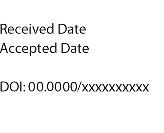
\includegraphics{auxiliary/rsc_template_head_foot/dates} & \noindent\normalsize{First commercial white light-emitting diodes (LEDs) were introduced to the market in 1996. Since then, white LEDs have experienced major improvements in performance and decreases in cost, resulting in rapid market expansion of LED-based solid-state lighting (SSL), one of the key current solutions in global climate change mitigation efforts. Despite the significance of the technology, the extent and sources of these improvements have not been systematically investigated. Understanding what has driven rapid progress in LEDs can provide lessons for accelerating innovation in a broad range of other demand-side clean energy technologies for climate change mitigation. With this aim, we gather systematic evidence on cost and performance improvements in white LEDs from a literature review, interviews with experts in industry and academia, and cost and performance modelling. We find that the overall efficiency of the highest performing warm white LED packages has improved from $\eta_L=5.8\%$ in 2003 to $\eta_L=38.7\%$ in 2020. During the same period, we estimate that the cost of manufacturing low-power and mid-power LED packages at a U.S. location using state-of-the-art equipment has dropped from 1.1\$ to 0.05\$ (in 2020 USD) between 2003 and 2020, a 95.5\% decrease. We also show that technology spillovers — i.e., knowledge originating in other technologies—affected all performance dimensions of LEDs, contributing no less than 8.5\% of the total efficiency improvements and $\sim$100\% of the improvements in consumer experience metrics. The increase in wafer size and manufacturing yield improvements were the primary causes of LED manufacturing cost reductions.}

\end{tabular}

 \end{@twocolumnfalse} \vspace{0.6cm}

  ]
%%%END OF TITLE, AUTHORS AND ABSTRACT%%%

%%%FONT SETUP - please do not change any commands within this section
\renewcommand*\rmdefault{bch}\normalfont\upshape
\rmfamily
\section*{}
\vspace{-1cm}


%%%FOOTNOTES%%%

\footnotetext{\textit{$^{a}$~ETH Zurich, Zurich, Switzerland. E-mail: michael.weinold@alumni.ethz.ch}}
\footnotetext{\textit{$^{b}$~Cambridge Centre for Environment, Energy and Natural Resource Governance, Department of Land Economy, University of Cambridge, Cambridge, United Kingdom. }}

%Please use \dag to cite the ESI in the main text of the article.
%If you article does not have ESI please remove the the \dag symbol from the title and the footnotetext below.
\footnotetext{\dag~Electronic Supplementary Information (ESI) available: [details of any supplementary information available should be included here]. See DOI: 00.0000/00000000.}
%additional addresses can be cited as above using the lower-case letters, c, d, e... If all authors are from the same address, no letter is required

\footnotetext{\ddag~Present address: Paul Scherrer Institut, Laboratory for Energy Analysis, Group for Technology Assessment, Switzerland.}


%%%END OF FOOTNOTES%%%

%%%MAIN TEXT%%%%

\section{Introduction}

A rapid reduction of global carbon dioxide emissions is urgently required in order to mitigate the effects of climate change \cite{Forster2019}. According to the United Nations, by the end of 2021, more than 130 countries have set or are considering setting a net zero emissions target by or around 2050 \cite{un2021climate}. The European Union, for example, has set a goal of net zero emissions by 2050—a goal it aims to meet with the help of the European Green Deal, alongside other EU and national policies \cite{eu2020green}. The United Kingdom similarly has adopted a similar strategy to achieve net-zero by 2050 \cite{noauthor_ieairena_2023}.

Achieving these ambitious and critically important targets will require both the deployment of new clean energy technologies, and the acceleration of innovation in existing supply-side \cite{sinn2012green} and demand-side energy technologies \cite{rgeVorsatz2009}. To ensure rapid adoption of these technologies, significant reductions in their costs and improvements in their performance and consumer experience are needed. This requires understanding how these cost reductions and performance improvements can be achieved \cite{Stephan2021} \cite{Ziegler2021}.

There are a range of mechanisms that contribute to improvements in a technology over time, including targeted research and development (R\&D) efforts, economies of scale, learning by doing \cite{Arrow1971}, and economies of scope \cite{johansson2012global}\cite{national2016power}\cite{iea2020perspectives}. The role of these factors at different stages of the innovation life cycle \cite{ grubler2012policies}, from research and technology development to demonstration, market formation and diffusion, is an area of active research \cite{Mowery1979} \cite{kavlak2018evaluating} \cite{Ziegler2021}. Innovation is also driven by forces of supply and demand. Various \textit{"technology-push"} drivers reduce the costs of innovating, while \textit{"market-pull"} drivers increase the pay-offs from investing in innovation \cite{anadon2009policy}.

\begin{figure*}[h]
 \centering
 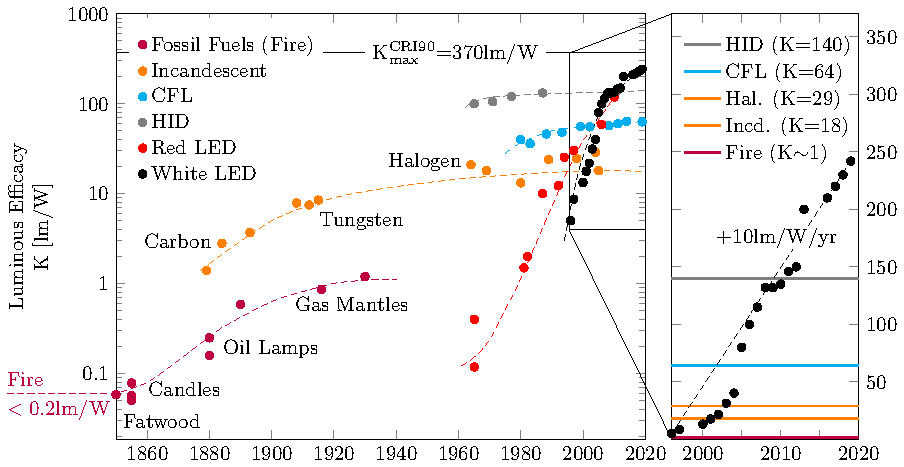
\includegraphics[height=7cm]{2_SSL_EES/article/figures/history_efficacy.pdf}
 \caption{Historical development of the luminous efficacy ($K$) of the most widely-used lighting technologies in human history from 1850 to 2020. Data shown for best performers by year of market introduction, with dashed lines. Dashed lines indicate the average improvement calculated from a 3rd-order polynomial fit to the data. The physical limit for an ideal light source with a colour rendering index of CRI=90, denoted as $K_max^{CRI90}$, is shown as a black horizontal line, as per calculations by Murphy et al. \cite{Murphy2012}. The magnified plot shows the progress in cool white LEDs from 1996 to 2020, with the dashed line indicating a linear rate of efficacy improvement of 10lm/W per year. For comparison, efficacies of best performers in legacy lighting technologies for 2020 are shown as coloured horizontal lines. Note the logarithmic scale of the vertical axis on the main plot and the linear scale on the magnified plot. Abbreviations: HID – High-Intensity Discharge; CFL – Compact Fluorescent Lamp; Hal. – Halogen, Incd. – Incandescent. Source: own synthesis of published data based on a visual approach proposed by Azevedo et al. \cite{azevedo2009transition}. See Supplementary Information, section , for the full list of data sources. }
 \label{fgr:history_efficacy}
\end{figure*}
 
 
The stages and drivers of the innovation life-cycle for a particular technology play out within a broader innovation system \cite{grubler2012policies}\cite{Anadon2016}. Among these drivers, the role of external  knowledge transfer and technology spillovers in research and development of energy technologies is an understudied area  \cite{Stephan2021}. While the exact definition of spillovers in literature depends on the context and the research question \cite{Liu2003}\cite{Nemet2012}, we follow Stephan et al. \cite{Stephan2021} and consider knowledge to be external – thus a spillover –  if it has been developed for application in other technologies, sectors, or scientific disciplines. There is emerging evidence that understanding spillovers and the knowledge network outside a technology may be an important factor in understanding \cite{Pichler2020} and shaping \cite{Clark2016}\cite{Stephan2021}\cite{Sun2021}\cite{kolesnikov_framework_2022} the future evolution of technologies.  

Among demand-side technologies, the provision of lighting is a particularly important area for climate change mitigation efforts, as it currently   accounts for 15-19\% of global electricity consumption \cite{Zissis2016}\cite{doe_electricity}. It is also an area of rapid recent technological change: since the introduction of the first commercial white light-emitting diodes (LEDs) in 1996, lighting technology has experienced dramatic efficiency improvements.  As shown in Figure \ref{fgr:history_efficacy}, thanks to the introduction of LED-based solid-state lighting (SSL), the efficacy of lighting sources has increased by three orders of magnitude in just over 20 years , which is significantly faster than the historical progress observed in previous lighting technologies \cite{weinold2021quantifying}. For comparison, the highest performing light-emitting devices today reach efficacies of 220 lm/W \cite{lumistrips2021mid}, while an incandescent light bulb can only reach efficacies of up to 18 lm/W. Moreover, this rapid improvement in efficiency has been accompanied by a similarly impressive decrease in LED manufacturing costs and retail prices. Figure \ref{fgr:cost_lamp_small} shows how LED retail prices have fallen by two orders of magnitude, at an annual price per flux decline during the period of from 2008-2020 of 27.3\%, in line with previous estimates \cite{Gerke2020}.  


\begin{figure}
\centering
  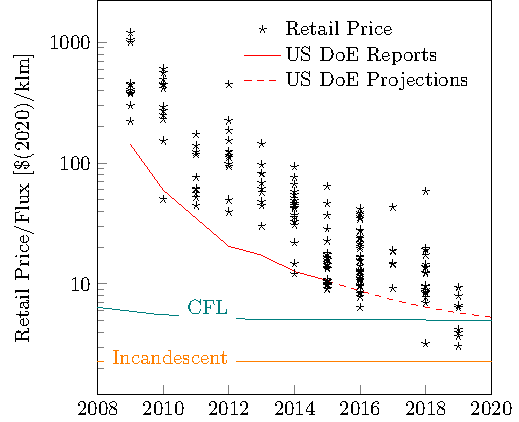
\includegraphics[height=6.5cm]{2_SSL_EES/article/figures/cost_lamp_small.pdf}
  \caption{Historical development of retail sales prices (in 2020 USD) per luminous flux of LED-based luminaires, including light bulbs, spotlights and recessed lights from 2008 to 2020. Red curved and dashed lines represent average retail sales prices and price projections for LED based luminaires published by the U.S. Department of Energy (DoE) \cite{council2013assessment}. Shown for reference are the average prices for compact fluorescent (CFL) and incandescent light bulbs. Source: own synthesis of data on LED sales prices collected from various consumer watchdog databases and publications. Data on CFL sales prices collected from \cite{eger2018origin} as well as various consumer watchdog databases and publications. Incandescent light bulb price is assumed constant based on the average in the covered time period. See Supplementary information, section …, for the full list of data sources.}
  \label{fgr:cost_lamp_small}
\end{figure}

These  dramatic improvements in lighting technology, supported by the introduction of lighting efficiency regulations phasing out incandescent lightbulbs and targeted policies stimulating LED adoption in many countries, led to the rapid expansion and diffusion of SSL technologies  \cite{weinold2020long}\cite{Mills2014}\cite{Stegmaier2021}\cite{grubb2021new}. As a result, by 2020, highly efficient LED luminaires were saving an estimated 131 TWh/year for the EU \cite{eu2019impactass} and 442 TWh/year for the US \cite{guidehouse2020adoption}, which is on par with the amount of energy produced annually by all solar photovoltaic installations in these regions. Notably, market adoption of LED lighting is not limited to developed economies \cite{Kamat2020}. For example, durability, low up-front cost and high efficiency of LED light sources have led to their wide-spread adoption in rural West African communities without access to grid electricity \cite{Bensch2017}. LEDs have also been used in a wide range of applications beyond lighting, such as personal health monitors \cite{o2019optical}, \cite{Wyatt2020}, watches and smartphones \cite{Bai2017}, potable water treatment \cite{Lui2014}, high-bandwidth wireless data transmission \cite{Haas2016}, and augmented reality eye wear \cite{Lee2016}. 

Despite this impressive history, the sources of LED innovation have not received as much attention from researchers as innovation in supply-side  energy technologies, such as solar photovoltaics  \cite{kavlak2018evaluating} or wind energy \cite{qiu2012price}\cite{jennings2020policy}, or in lithium-ion batteries for transportation \cite{Ziegler2021}\cite{Stephan2021}. To the best of our knowledge, no study has comprehensively discussed the sources or extent of progress across various metrics of LED cost or performance since the introduction of first commercial white LED products.  Understanding the extent to which individual innovations and knowledge spillovers  contributed to improvements in LED technology, how this effect compares to other sources of improvements such as economies of scale, and how these innovations occurred (i.e., by what mechanisms and actors) will provide valuable lessons both for other demand-side technologies and overall for accelerating clean energy innovation.

To address these questions, in this paper we identify a set of metrics suitable for tracking the historical progress of LED lighting technology. We then trace device efficiency and cost improvements, as well as changes in relevant consumer experience metrics from the time of introduction of the first commercial warm white LEDs in 2003 to 2020, the year with the most recent data available at the time of writing  . Given the proprietary nature of knowledge in the SSL industry , we collect corresponding information using a multi-method approach combining a systematic literature review of scientific literature and industry reports with patent analysis and a series of elite interviews \cite{Tansey} with eminent experts from academia, public research institutions and industry. This approach allows us to identify innovations in white LED technology and examine their origins to discern technology spillovers among them. Data on performance improvements associated with individual innovations identified in patents, scientific publications, industry reports, and interviews is then augmented  by our calculations of device efficiency, including contributions of specific spillovers to the overall LED efficiency (see Supplementary Information for more detail). We further calculate LED manufacturing costs using own bottom-up cost model with a process-step resolution. Finally, we discuss what our observations and conclusions mean for the understanding of the innovation process in LED technology and for broader policy and industry efforts to accelerate clean energy innovation.

\section{Previous literature}

The historical development of light-emitting diodes has received a considerable amount of attention following the recognition of pioneering work on blue LED by Japanese researchers Shuji Nakamura, Isamu Akasaki and Hiroshi Amano with the 2014 Nobel Prize in Physics \cite{Akasaki2015}\cite{Nakamura2015}. The sources and disaggregated contributions of subsequent improvements in LED technology, however, have not been documented in the literature in a systematic fashion, though there were notable publications reporting on the progress in the design of devices \cite{Shchekin2006}\cite{krames2007led}\cite{laubsch2009high}\cite{hahn2014development}, or the technological improvements  underlying the improvement in overall device efficiency for best performers in 2009 \cite{tsao2010solid} and 2016 \cite{pattison2017solid}. 

Several descriptive publications provide a very useful overview of some of the scientific breakthroughs  that have contributed to LED progress \cite{krames2007status}\cite{Phillips2007}\cite{Bierhuizen2007}\cite{Nakamura2013}\cite{feezell2018invention}\cite{Taki2019} . Additional  studies providing more detail the origin and impact of specific advances in LED technology as well as their integration into device manufacturing were published by authors working for key industry actors Lumileds\cite{MuellerMach2005}\cite{Shchekin2006}\cite{lumi2015lumi}\cite{Bhardwaj2017} and Osram (now amsOsram) \cite{Haerle2004}\cite{Baur2009}\cite{laubsch2009high}\cite{hahn2014development}. However, these studies typically include limited information on the macro-level chip-design and cover disparate aspects of the technology over different time periods. Another important source of historical information comes from patents, which cover the entirety of the device architecture or manufacturing process, including those by Lumileds \cite{margalith2011thin}, Samsung \cite{jung2014phos} \cite{cha2019semiconductor} and Soraa \cite{cich2017high}.

We summarize the information collected, analysed and classified on the progress in LED chip architectures and manufacturing processes from these and other disparate sources in Figure \ref{fgr:chip_architecture_overview}, where we show the evolution of LEDs from classical chips with lateral current spreading to chip-scale package flip-chip architectures. Despite the amount of literature published on the topic of LED history, to the best of our knowledge, no publication comprehensively aggregates known chip design, manufacturing, and material improvements to show the overall effect of these improvements on device efficiency or manufacturing cost over time. In addition, the effect of individual innovations and technology spillovers, which has been investigated in solar PV \cite{kavlak2018evaluating}\cite{kolesnikov2020novel}\cite{nemet2019solar}, and to some extent in lithium-ion batteries \cite{Stephan2021}, has not been studied in the context of lighting yet. This is consistent with previous observations regarding the marginalization of end-use technologies in the analysis of energy innovation for climate change impact mitigation \cite{Wilson2012}\cite{Creutzig2018}.


\begin{figure*}
 \centering
 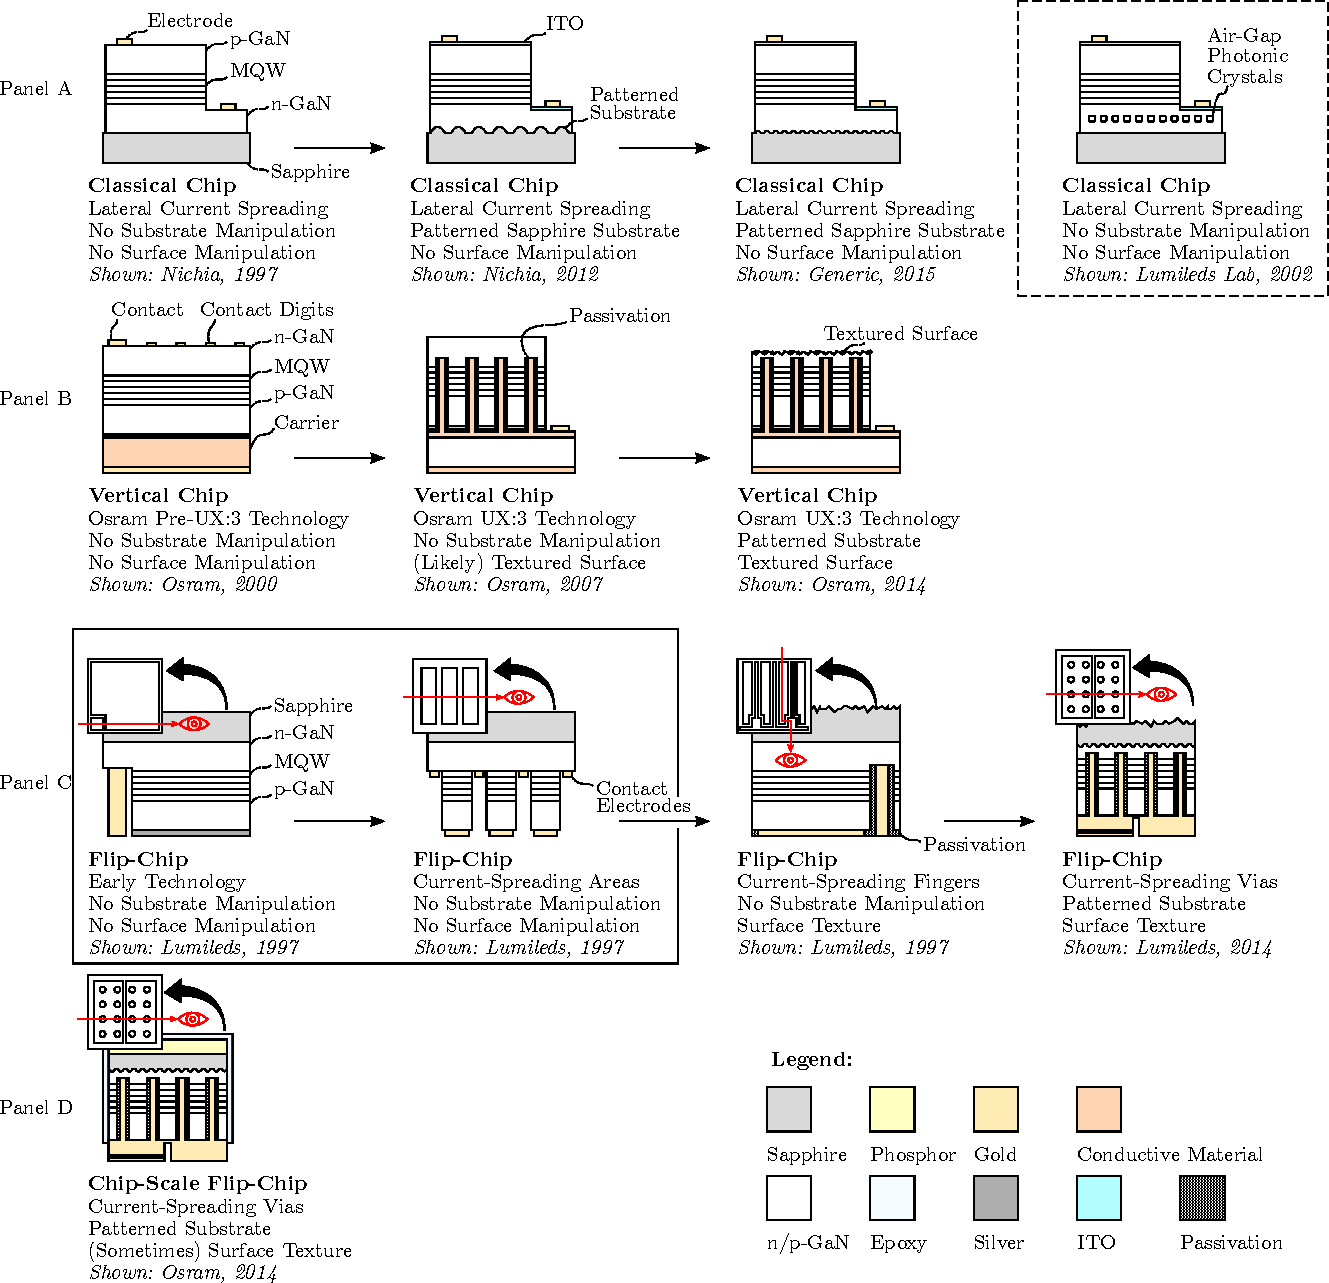
\includegraphics[height=17cm]{2_SSL_EES/article/figures/chip_architecture_overview.pdf}
 \caption{Historical evolution of light-emitting diode chip architectures. Rows from top to bottom: classical chip with lateral current spreading; Osram’s thin GaN flip-chip (vertical) architecture; flip-chip architecture; chip-scale package flip-chip architecture. Shown are side views of chips without packages, along a cutaway line best suited to the features of each architecture. The cutaway surface is indicated by a red arrow with an eye on the overlaid top view of each chip. Note that the dimensions are not to scale, and smaller features are greatly exaggerated for clarity. Years indicated correspond to the earliest identified patent priority date. Black frames around certain designs indicate chip designs not brought to large-scale production. Abbreviations: GaN – Gallium Nitride, ITO – Indium Tin Oxide, MQW – Multiple Quantum Well. Source: adapted and compiled from multiple patents and industry publications. See Supplementary Information, section…, for the full list of sources and references.}
 \label{fgr:chip_architecture_overview}
\end{figure*}

\section{Metrics for technological progress in LEDs}

Investigating the sources of rapid progress in LED technology over the past decades, in which white LEDs have come to dominate the lighting market \cite{zissis2021}, requires selecting appropriate metrics for tracking and quantifying this progress. The choice of metrics affects both what data sources can be used in the analysis and which research methodologies can be used to calculate and analyse such metrics. We select the metrics based on the following two general criteria. First, we focus only on metrics widely accepted and reported in industry because metrics proposed in the scientific literature but not reported by device manufacturers cannot be used to compare the performance of commercial LED devices over time. Second, the chosen metrics must be useful for understanding the impact of individual technological improvements on relevant performance and cost characteristics.

Historically, the progress in LED technology is commonly described by pointing to impressive improvements in LED device performance (i.e., brightness and electrical efficiency) and manufacturing cost reductions \cite{Taki2019}. However, solid-state lighting performance is characterized not only by LED brightness or electrical efficiency. Consumer experience, including the perceived temperature of a white light source and its ability to faithfully render colours, has also played a significant part in the market adoption of new lighting technologies \cite{Menanteau2000}\cite{Sandahl2006}\cite{CAIRD2008}\cite{murphy2012governing} and received substantial attention in LED research and development efforts \cite{azevedo2009transition}\cite{cho2017white}. Therefore, a comprehensive analysis of the evolution in white LED technology must take into consideration advances in: 1) physical device performance; 2) consumer experience; and 3) LED device manufacturing costs. Next, we introduce and discuss the metrics that we use to track progress in each of these three areas. 

\subsection{Device Performance Metrics}
\label{sec:device_performance_metrics}

Initially, as LED devices developed, the primary metric of progress in solid-state lighting was typically the luminous flux, as reflected in the so-called “Haitz’s Law” \cite{haitz1999case}\cite{haitz2011solid}. The luminous flux (total brightness) of early white LEDs was too small to allow for the economical combination of multiple LEDs into lamps for general illumination purposes. In 2000, highest performing devices yielded around 10lm, just below the output of a candle as defined in the unit candela (1cd=12.57lm) \cite{haitz2011solid}. Today, however, highest performing devices yield in excess of 1600lm, the equivalent of a 100W incandescent bulb \cite{cree2020bright}. LED brightness has become sufficient to enable the construction of lamps from multiple LED devices, with design improvements focusing on higher efficiency and quality of light instead of brightness. Even though some scientific publications and industry periodicals continue to focus on brightness as a metric of progress in lighting, we find that, by now, it fails to capture the complexity of the multitude of efficiency improvements that have been driving overall LED efficiency \cite{weinold2021compound}. 

\subsubsection{Forward Voltage Efficiency $\eta_{V_f}$}

Device forward voltage efficiency\footnote{"Joule Efficiency" $\epsilon_J$ in Tsao et al. \cite{tsao2010solid}} $V_fE$ describes all electrical losses at the interface between the electrodes and the semiconductor and in the bulk. These losses can be due to tunneling and Ohmic resistance at the interface, as well as Ohmic resistance and other electrical losses within the bulk of the semiconductor. It is defined as

\begin{equation}
    \eta_{V_f} = \frac{E_{h\nu}}{V_f}
\end{equation}

where $E_{h\nu}$ denotes the photon energy and $V_f$ is the diode forward voltage \cite{schubert2018light}\cite{tsao2010solid}.

\subsubsection{Light Extraction Efficiency $\eta_{LE}$}

Device light-extraction efficiency describes the  losses due to absorption in the material after electron-hole recombination and the associated emission of a photon. It is defined as

\begin{equation}
    \eta_{LE}=\frac{\text{\# of photons out}}{\text{\# of photons created}} = \frac{P_{opt}}{P_{int}}
\end{equation}

where $P_{opt}$ is the optical power of the device and $P_{int}$ is the internal power of the device\cite{schubert2018light}\cite{tsao2010solid}.

\subsubsection{Internal Quantum Efficiency $\eta_{IQ}$}

Internal quantum efficiency describes non-radiative recombinatory processes in the semiconductor bulk. It is related to the external quantum efficiency through
\begin{equation}
\label{eqn:ieq-eqe}
    \eta_{EQ} = \eta_{IQ} \times \eta_{LE}
\end{equation}

and defined as

\begin{equation}
    \eta_{IQ} = \frac{\# \text{of photons created}}{\# \text{of electron-hole pairs in}}
\end{equation}

and depends on the current density of the device\cite{schubert2018light}\cite{tsao2010solid}. 

\subsubsection{Droop $\eta_{droop}$}

(Efficiency) droop describes the decrease of device internal quantum efficiency at high current densities, which is caused by a number of different physical effects\cite{David2020}. This is often treated separately from internal quantum efficiency in literature due to its importance in high-power devices. It is defined as

\begin{equation}
    \eta_{droop} = 1 - \frac{\eta_{IQE}}{\eta_{IQE}(A \rightarrow 0)}
\end{equation}

where $\eta_{IQE}(A \rightarrow 0)$ denotes the internal quantum efficiency at low current densities. In practice, droop is often given as the percentage difference between the ideal luminous intensity curve $\phi_{ideal}$ and the real luminous intensity curve $\phi$ at a set diode test current $A_{test}$ as

\begin{equation}
\label{eqn:droop}
    D = \frac{\phi_{ideal}(A_{test})-\phi(A_{test})}{\phi_{ideal}(A_{test})/100}
\end{equation}

Thereby, according to this definition, a lack of droop corresponds to a droop efficiency of $\eta_{droop} = 100\%$\cite{schubert2018light}\cite{tsao2010solid}.

\subsubsection{Conversion Efficiency $\eta_{C}$}

(Light) conversion efficiency describes losses in the conversion process of blue light that is the basis for all phosphor-converted white LEDs. These losses are the sum of the Stokes loss and well as scattering/absorption losses. It is defined as

\begin{equation}
    \eta_{C} = \frac{E_{\textcolor{blue}{B}}}{\sum_{i=\textcolor{red}{R},\textcolor{orange}{O},\textcolor{yellow}{Y},\textcolor{teal}{G}} E_i}
\end{equation}

where $E_i$ denotes the total energy of light at the color corresponding to the down-converted photon wavelength (Blue, Red, Orange, Yellow, Green)\cite{schubert2018light}\cite{tsao2010solid}.

\subsubsection{Spectral Efficiency $\eta_{S}$}

Spectral efficiency describes losses in the conversion process due to the wavelength-dependent efficiency of the human eyes. Photons converted into the infrared or ultraviolet are lost to illumination purposes. It is defined as

\begin{equation}
    \eta_{S} = \frac{K}{K_{max}(CRI,CCT)}
\end{equation}

where $K$ is the luminous efficacy of radiation of the light source, can be computed from the spectrum and the luminosity function, which describes the sensitivity of the human eye.$K_{max}$ is the maximum luminous efficacy of radiation of a perfect light source with the same color rendering performance and correlated color temperature as the light source in question\cite{schubert2018light}\cite{tsao2010solid}. 

\subsection{Consumer Experience Metrics}

The perceived quality of light is entirely determined by the emission spectrum of a light source \cite{ies_handbook}. Any metric relevant to customer experience can thus be calculated from the spectrum alone. The spectrum of an LED light source is determined by the emission wavelength of the LED itself and the absorption and emission spectra  of the downconversion phosphor used in the device. It is typically included in the product datasheets provided by manufacturers, which enables the calculation of all relevant spectrum-based metrics for these devices. Based on the prevalence in scholarly literature and industry publications, for this study we choose two consumer experience metrics: Colour Rendering Index (CRI) and Colour Temperature. We do not consider flicker, the unintended high-frequency temporal modulation of light, which is another important consumer experience metric for lighting and a subject of recent regulation by the European Union /cite{weinold2020long}. This effect is caused not by LEDs themselves, but rather by inadequately designed electrical ballasts \cite{Lehman2014}. It is thus beyond the scope of this work. 

The Colour Rendering Index (CRI) of a light source describes its ability to render the colours of an object faithfully when compared to illumination under a reference light source, such as standard daylight \cite{khan2015led}. The way it is calculated is defined by the International Illumination Commission (CIE) \cite{cie_cri_1995}. CRI has certain limitations when applied to solid-state light sources \cite{david2013cri}. However, despite repeated attempts at constructing more elaborate colour rendering metrics \cite{Houser2013}, CRI has remained the de-facto industry standard for describing colour fidelity of light sources \cite{DoE2016LED}. High colour rendering performance of lighting is a requirement in workplace environments, retail stores, clinical operating environments and art exhibitions \cite{khanh2017color}. It should be noted that some niche applications prioritize high colour saturation over high CRI, for instance, in food display or fabric retail applications \cite{david2013cri}. However, these niche applications remain outside our focus on general illumination. Due to a broad availability and importance of CRI data for consumers of various LED lighting sources, we adopt CRI as the key metric to track progress in consumer experience in LED lighting, despite its limitations. 

The Colour Temperature of a light source describes the equivalent temperature of an ideal black body which emits light of a colour comparable to that of the light source \cite{commission2011cie}. Warm white light sources are widely used in general illumination, while cold white light sources are used in workplace illumination and outdoor lighting. Early white LEDs produced only cool white light \cite{mueller2000light}. The introduction of first commercial warm white LED light bulbs played a significant part in increasing adoption of LED-based lighting among consumers, as their spectrum more closely resembled the warm white colour temperature of incandescent light bulbs \cite{al2016optics}. For this reason, we also adopt colour temperature as a metric for tracking progress in consumer experience in LED lighting.

\subsection{Manufacturing Cost}

In selecting metrics for tracking the progress in manufacturing cost reductions in LED, we must first highlight  the complexity of this task. Access to manufacturing cost data at the chip level is usually restricted due to its proprietary nature and is available only for selected products. Using sales price information instead of the cost for the same purpose could be in some cases a promising alternative, as prices can be easily obtained for recent LED products directly from manufacturers. However, historical data on prices for LEDs is as difficult to obtain as for costs. In addition, sales price includes components not relevant to the progress in technology, such as profit margins and overhead costs, and is affected by policies such as rebates and purchase subsidies. Historical information on these factors and price components, as well as their impact on the manufacturing cost for each LED product under consideration is even harder to obtain, making the use of LED sales prices as a direct metric of technology progress very difficult in practice. 

\section{Methods and Data Collection}

The evolution of LED device architecture and performance as well as the progress in understanding the underlying physical phenomena are well covered in the scholarly literature and patents, as described in section 2. However, information provided in such sources is insufficient for our goals on at least three accounts. First, existing work focusses  only on selected performance parameters or overall device efficiency, rather than on providing a comprehensive coverage of the whole device sub-efficiencies for a particular LED product or design. Scientific publications also do not always disclose the underlying device architecture or the features responsible for the gains in performance. Second, not all relevant innovations are patented \cite{Pakes_1980}\cite{ Fontana_2013}. In the case of LED patents in particular, our interviews with industry experts suggest that the propensity to patent is the highest for knowledge related to macroscopic device architecture and chemical composition of phosphors, and the lowest for knowledge related to manufacturing process improvements and microscopic chip architecture that is difficult to reconstruct by reverse engineering. This means that relying only on patent literature would bias results by unduly emphasizing some focus areas and de-emphasizing others. Third, scientific publications and patents typically focus on experimental devices, rather than commercial products. While new LED features, designs and manufacturing methods reported in these sources can potentially result in significant performance gains or cost reductions, it is difficult to ascertain if these improvements have since been adopted in industry.  Furthermore, information on LED manufacturing cost and the effect of process improvements on the total cost is highly proprietary. Estimates are occasionally reported in the scientific literature and company publications, but these often do not disclose which parts of the manufacturing process are responsible for the largest contribution to the overall cost, or which improvements led to cost reductions.

To overcome the limitations of these different methods for understanding technological progress, in this study we rely on a multi-method approach to data collection and analysis that combines information obtained from a review of the primary scientific literature and relevant patents with our own computations of device sub-efficiencies, information gained from industry publications, semi-structured interviews with experts from academia and industry, and bottom-up manufacturing cost modelling. We provide the details of implementation of each of these methods below.

\subsection{Systematic Literature Review}

We collected data on LED performance and characteristics in a systematic literature review that included scientific publications, patents, conference proceedings from the largest semiconductor and optoelectronics conferences, industry periodicals and roadmaps, as well as company presentations and reports. This review was structured around the three main goals: 1) tracking the evolution of LED technology over time as indicated by three groups of progress metrics selected above in the “Metrics” section; 2) identifying individual innovations that contributed to this evolution and whether or not they could be spillovers, and quantifying their impact on device performance and manufacturing cost; and 3) determining whether these innovations had originated within the LED technology domain, or in a field of research or technology outside of solid-state lighting, making them a technology spillovers. 

Relevant  sources for the review were found in an iterative search process that involved two components. The first was the search in specialized patent and publication databases such as Google Scholar, Google Patents, and Scopus , as well as company websites. The second component was the analysis of backward citations in the identified sources, starting from the reviews mentioned in the “Previous literature” section and then iteratively repeating it for all newly identified sources, until no further relevant and significant new sources were found. We also relied on backward citations for the identification of technology spillovers,   considering cited documents as indicators of knowledge origins of an innovation and analyzing whether those documents belonged to the LED technology domain or not.

\subsection{Semi-Structured Interviews}

To supplement our data collection efforts, verify our findings and identify additional spillovers, we conducted a series of elite semi-structured interviews with eleven eminent experts  from academia, industry and public research sector . Experts were selected based on their engagement in  different sub-fields of LED research and manufacturing, as well as the recommendations from other interviewed experts, in essence expanding the list of experts that emerged from the literature review by what is known as a snow-ball sampling method. All interviews were conducted between November 2019 and April 2022 by means of video conferencing and lasted for about one hour. A summary of the background of interviewed experts is provided in Table X in the supplementary information.

The primary, structured part of the interviews explored which innovations were deemed most relevant to the evolution of device performance, consumer experience and manufacturing cost of LED packages. Thereafter, interviewees were asked to consider the extent to which these innovations may have originated outside of their respective field of expertise and the LED industry more broadly—i.e., which of the innovations may be considered spillovers. The remainder of the interview was focused on learning about particular aspects of the manufacturing processes relevant to cost and performance modelling, the current state of industry, and the circumstances surrounding the innovations and spillovers identified in the first part of the interview. Specific quantitative data was also provided by experts, helping fine-tune the parameters of the manufacturing cost model (described in subsection 4.4) and verify device performance data.

\subsection{Performance Metrics Calculations}

The contribution of individual technology innovations and spillovers to the progress in the overall device efficiency over time is estimated by the index decomposition analysis, which is commonly used in energy economics \cite{Ang2019}. Specifically, we use the additive logarithmic mean Divisia index method I (LMDI-I), also known as the Additive Sato-Vartia indicator \cite{deBoer2019}. It was developed by Boyd in 1987 \cite{Boyd1987} on the basis of Divisia index, a method in statistical economics \cite{Diewert1988}, and subsequently refined \cite{Ang1997}.

\section{Results}

\begin{figure*}[h!]
 \centering
 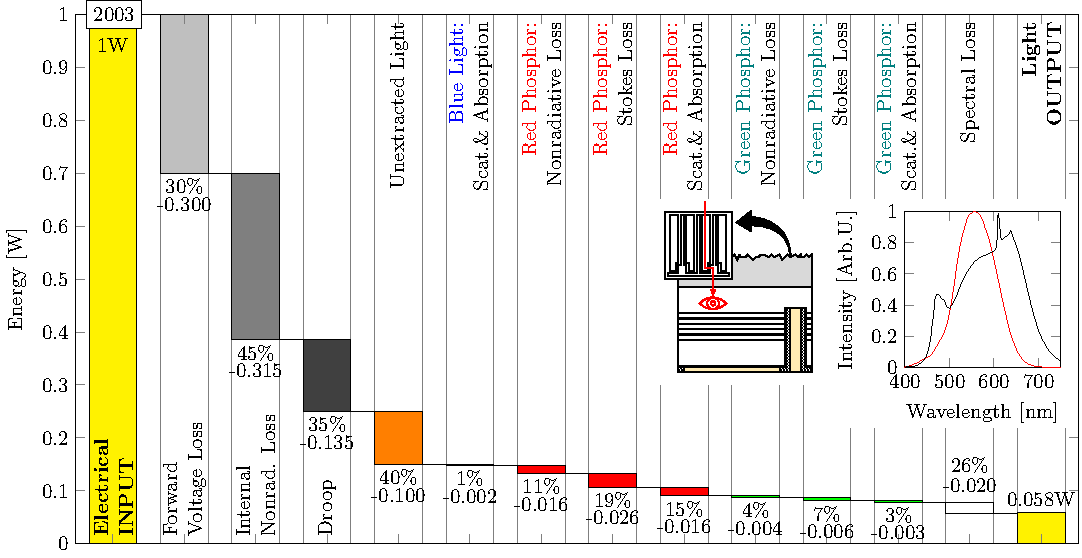
\includegraphics[width=16.5cm]{2_SSL_EES/article/figures/waterfall_performance_2003.pdf}
 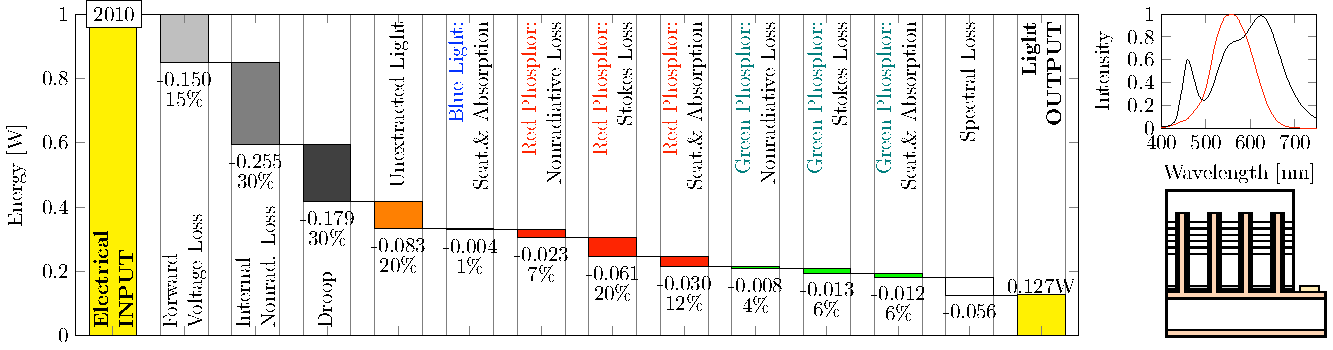
\includegraphics[width=16.5cm]{2_SSL_EES/article/figures/waterfall_performance_2010.pdf}
 \caption{Waterfall diagrams of the loss channels in a generic mid/high-power LED package for 2003 (top panel) and 2010 (bottom panel), normalized to 1 Watt of electric power input (yellow bar on the left). Sub-efficiencies corresponding to each loss channel are listed below each column and described in Section \ref{sec:device_performance_metrics}. Numbers for each loss channel indicate energy losses both in relative terms of input power (in percent) at the point of the channel and absolute values (in Watts). Percentages for red, green and blue loss channels indicate losses of remaining red/green/blue light energy. The following corresponding LED architectures from Figure \ref{fgr:chip_architecture_overview} are shown for reference: 2003 (top panel) – flip-chip with YGAG phosphor; 2010 (bottom panel) – flip-chip with 258 phosphor. Details on phosphors are provided in Table XX and SI section XX. Overall LED package efficiency is $\eta_L = 5.8\%$ in 2003 and $\eta_L = 12.6\%$ in 2010. Abbreviations: Scat. = Scattering. Source: own elaboration based on data from sources listed in SI, section XX.}
 \label{fgr:waterfall_1}
\end{figure*}

\section{Conclusions}
Our study has analysed in a systematic and granular way the sources of dramatic cost reductions and efficiency improvements in white light-emitting diodes since their introduction to the market in 1996. We find that the total LED device efficiency increased from $5.8\%$ to $38.7\%$ between 2003 and 2020 has been predominantly driven by LED technology innovations that have affected all physical energy loss channels and corresponding device sub-efficiencies. We also find that among those innovations, at least nine were driven by technology originating in areas of science and technology outside LEDs and solid-state lighting—i.e., those nine innovations can be referred to as technology spillovers . These spillovers were responsible for $8.5\%$ of the total efficiency improvements and nearly $100\%$ of the improvements in consumer experience metrics. 

Our manufacturing cost model shows that a $95.5\%$ decrease in the cost of producing white classic-chip LEDs (from $1.11\$$ to $0.05\$$ in 2020 USD) between 2003 and 2020. While efficiency improvements have played an important role in these cost reductions, the largest components of such cost reductions have been driven by increases in the wafer size and yields across different manufacturing steps. In contrast with efficiency improvements, these increases were mainly a result of learning-by-doing and manufacturing equipment improvements rather than LED technology innovations or spillovers. 

Our analysis of the sources, mechanisms and enablers of the identified technology spillovers which were significant drivers of efficiency improvements, highlights the critical role played by a growing deep understanding of the physical, chemical and optical phenomena underlying the operation of LEDs, as well as materials science and technology and nanotechnology involved in the production of LEDs. Specifically, deep physical understanding of LED device efficiency loss channels enabled important breakthroughs and spillovers in LEDs and will enable further innovations to improve LED and SSL efficiency in the future, as expected by eminent experts in the field \cite{Weisbuch2020}. This suggests that additional research in these areas and a more deliberate search for spillovers may accelerate these expected future advances. Our findings on spillover enablers show that these efforts can be further supported or even accelerated by knowledge exchange events and long-term partnerships between academia and industry, dedicated mission-driven public R\&D funding, and freedom of search in academia. This reinforces arguments made against the dichotomy of basic research versus applied research \cite{narayanamurti2016cycles} \cite{narayanamurti2021genesis} and the calls for open, inclusive and flexible research cultures \cite{Stephan2021}.

There are various important avenues of future research that are opened up by our analysis. First, future work could expand the cost model by collecting and including data for a broader set of chip architectures and analyzing the impact of individual innovations and spillovers on costs as opposed to performance. Second, a deeper dive on the role of learning-by-doing is needed both in the cost and performance analysis to identify different types of learning by doing and how it came about. Third, building on the work on LED sub-efficiencies and physical limits, future efforts could focus on identifying priority areas for further efficiency improvements in LEDs and SSL in general. Finally, by comparing the drivers of innovation, technology spillovers, cost reductions and performance improvements at a granular level across different clean energy technologies, we can identify patterns or differences that would help us formulate recommendations for industry and policymakers aimed at accelerating further clean energy innovation for climate change mitigation. 

\section*{Conflicts of interest}
There are no conflicts to declare.

\section*{Acknowledgements}
This research is supported by the grant from the Alfred P. Sloan Foundation titled \textit{“What factors drive innovation in energy technologies? The role of technology spillovers and government investment”}. Michael Weinold further gratefully acknowledges financial support from the Swiss Study Foundation. We would like to thank Venkatesh Narayanamurti, Gabriel Chan, Anna Goldstein, Didier Sornette, and participants of the SPIE West 2021 Conference and C-EENRG Seminar Series of the University of Cambridge for many helpful discussions and feedback. We also express our deep gratitude to all interviewees for their willingness to participate in this study and their invaluable contributions.

%%%END OF MAIN TEXT%%%

%The \balance command can be used to balance the columns on the final page if desired. It should be placed anywhere within the first column of the last page.

\balance

%If notes are included in your references you can change the title from 'References' to 'Notes and references' using the following command:
%\renewcommand\refname{Notes and references}

%%%REFERENCES%%%
\bibliography{bibliography}
\bibliographystyle{auxiliary/rsc_style_files/bibliography_rsc} %the RSC's .bst file

\end{document}
